\documentclass[10pt,twocolumn,letterpaper]{article}
%\usepackage[latin1]{inputenc}

%\usepackage{url}
%\usepackage{booktabs}

\usepackage{cvpr}
\usepackage{times}
\usepackage{epsfig}
\usepackage{graphicx}
\usepackage{amsmath}
\usepackage{amssymb}
\usepackage{amsmath}
\usepackage{amsfonts}
\usepackage{subfigure}
\usepackage{nonfloat}
\usepackage{url}
\usepackage[colorlinks=true, linkcolor=green, pagebackref]{hyperref}
\usepackage{textcomp} % for textonehalf
%\usepackage{subref}
\graphicspath{{imgs/}}

\usepackage{xspace}
\renewcommand*{\eg}{e.g.\@\xspace}
\renewcommand*{\ie}{i.e.\@\xspace}
\newcommand*{\ea}{et al.\@\xspace}
%\renewcommand{\arraystretch}{1.5}

%\cvprfinalcopy % *** Uncomment this line for the final submission

\def\cvprPaperID{****} % *** Enter the CVPR Paper ID here
\def\httilde{\mbox{\tt\raisebox{-.5ex}{\symbol{126}}}}

% General noration
\newcommand{\prob}{Pr}
\newcommand{\degree}{^{\circ}}

% Image notation
\newcommand{\rgbdimage}{\mathcal{D}}
\newcommand{\intrinsics}{K}

% Voxel notation
\newcommand{\voxelgrid}{V}
\newcommand{\voxel}{\mathbf{v}}
\newcommand{\voxidx}{i}
\newcommand{\voxelidxs}{m, n, l}

% Point cloud notation
\newcommand{\pcloud}{\mathcal{P}}
\newcommand{\point}{\mathbf{p}}
\newcommand{\normal}{\mathbf{n}}

% Transformations
\newcommand{\trans}{T}
\newcommand{\extrinsics}{H}
\newcommand{\voxelgridtoworld}{\trans_{\voxelgrid \rightarrow w}}


\definecolor{red}{rgb}{0.95,0.4,0.4}
\definecolor{blue}{rgb}{0.4,0.4,0.95}
\definecolor{darkred}{rgb}{0.8,0,0}
\definecolor{darkgreen}{rgb}{0,0.5,0}
\definecolor{grey}{rgb}{0.6,0.6,0.6}

\newcommand{\todo}[1]{\textcolor{red}{TODO: #1}}
\newcommand{\note}[1]{\textcolor{blue}{NOTE: #1}}
\newcommand{\status}[1]{\textcolor{blue}{Status: #1}}
\newcommand{\add}[1]{\textcolor{darkgreen}{#1}}
\newcommand{\remove}[1]{\textcolor{grey}{#1}}



%[citecounter=true, style=ieee]
%\usepackage{biblatex}
%\addbibresource{bibtex/strings.bib}
%\addbibresource{bibtex/main.bib}
%\addbibresource{bibtex/crossrefs.bib}
%addbibresource{\jobname.bib}


\title{Predicting the Occupancy of Unobserved Voxels From a Single RGBD Image}

%\author{Michael Firman, Gabriel Brostow, Simon Julier \ea}

\begin{document}


\maketitle

\begin{abstract}
	Gaining a representation of the geometry of a scene is an essential task for many applications including robotic navigation, scene re-lighting and object manipulation. 
	Most existing works to recover the scene geometry rely on combining multiple views of the scene captured from many different directions or use of \emph{a priori} information about the expected semantic make-up of the scene.

	%We present a method to predict whether or not each voxel in a scene is occupied given just a single RGBD image.
  We are interested in recovering information about the 3D shape of a scene given an image captured from a single viewpoint.
  To do this, introduce a method to predict the occupancy of voxels which are not directly observed by the camera.
	We argue that objects of dissimilar semantic classes often share similar shapes; this allows for a limited training dataset to model the shape of a wide range of objects and hence estimate the hidden geometry of arbitrary scenes.

	Our primary contribution is the \emph{voxlet}, a primitive explaining voxel occupancy in the region of a point in 3D space. We also develop a novel feature representation, which coupled with a Random Forest forms a mapping from a point in a depth image to a prediction of voxel occupancy in the point's vicinity.
  We present a range of qualitative and quantitative results which show we can accurately reconstruct shape in both simple and challenging scenes, and we show many advantages over the current state-of-the-art.
%  We demonstrate the advantages of our technique over the current state of the art.

  %, method comprises of three main components:
   % 1) We generate a dinctionary of voxlets, which is a primitive describing 
   % 2) We introduce a novel regional feature to describe the shape of the region surrounding a point.
    %3) We use a Random Forest, trained on turntable and real-world data to map our feature representations of a pixel to a suitable voxlet which can be used to describe local voxel occupancy.
    %4) Finally we combine and regularise the  predictions to form a full probabilistic distribution of occupancy for each voxel in the scene, respecting constraints such as connectivity and gravity.

\end{abstract}

%%%%%%%%%%%%%%%%%%%%%%%%%%%%%%%%%%%%%%%%%%%%%%%%%%%%%%%%%%%%%%
\section{Introduction}
%%%%%%%%%%%%%%%%%%%%%%%%%%%%%%%%%%%%%%%%%%%%%%%%%%%%%%%%%%%%%%

Each location in our 3D world can be classified as being either `occupied' by a solid, or `vacant' and passable.
Depth cameras such as the Microsoft Kinect are able to give an estimate of which regions of a scene are composed of free space.
However, each pixel in a depth image only makes a prediction of occupancy until the first solid surface is encountered along that camera ray.
The `occlusion phenomenon' prevents any information to be extracted about the occupancy of space beyond that first surface.

There has been much research in vision in going from 2D images and depth images to reconstructing the full shape of our 3D world.
Many approaches rely on the fusion of images of a scene or object captured from multiple viewpoints \cite{izadi-uist-2011, vicente-cvpr-2014}, effectively bypassing the effect of occlusion.
Instead, we focus on the task of classifying each voxel in a 3D scene as being either `occupied' or `vacant' given just a single depth image from one viewpoint (figure \ref{fig:intro}).

%The set of use cases for such a 3D reconstruction from a single image is large and diverse.
There are many different applications for such a 3D reconstruction from a single image.
When a robot sets out to grasp an unknown object in an unknown environment, it is unlikely to be able to grip the object solely on the visible face: Instead the `fingers' of the robot hand must extend into unseen regions of the scene.
A 3D model of the immediate environment can be used to enable this grasping to take place without colliding with the object or nearby clutter.
In graphics, adding a new light source to an image after it has been captured can be a laborious and challenging task due to the many shadows and highlights which are typically manually added to the scene.
A full 3D model of the scene can allow for the automated addition of realistic shadows using ray-tracing techniques, making such operations easier to effect.

\newcommand{\introsubwidth}{0.48\columnwidth}
\begin{figure}[!t]
    \centering 
    \subfigure[Voxel world model]{%
        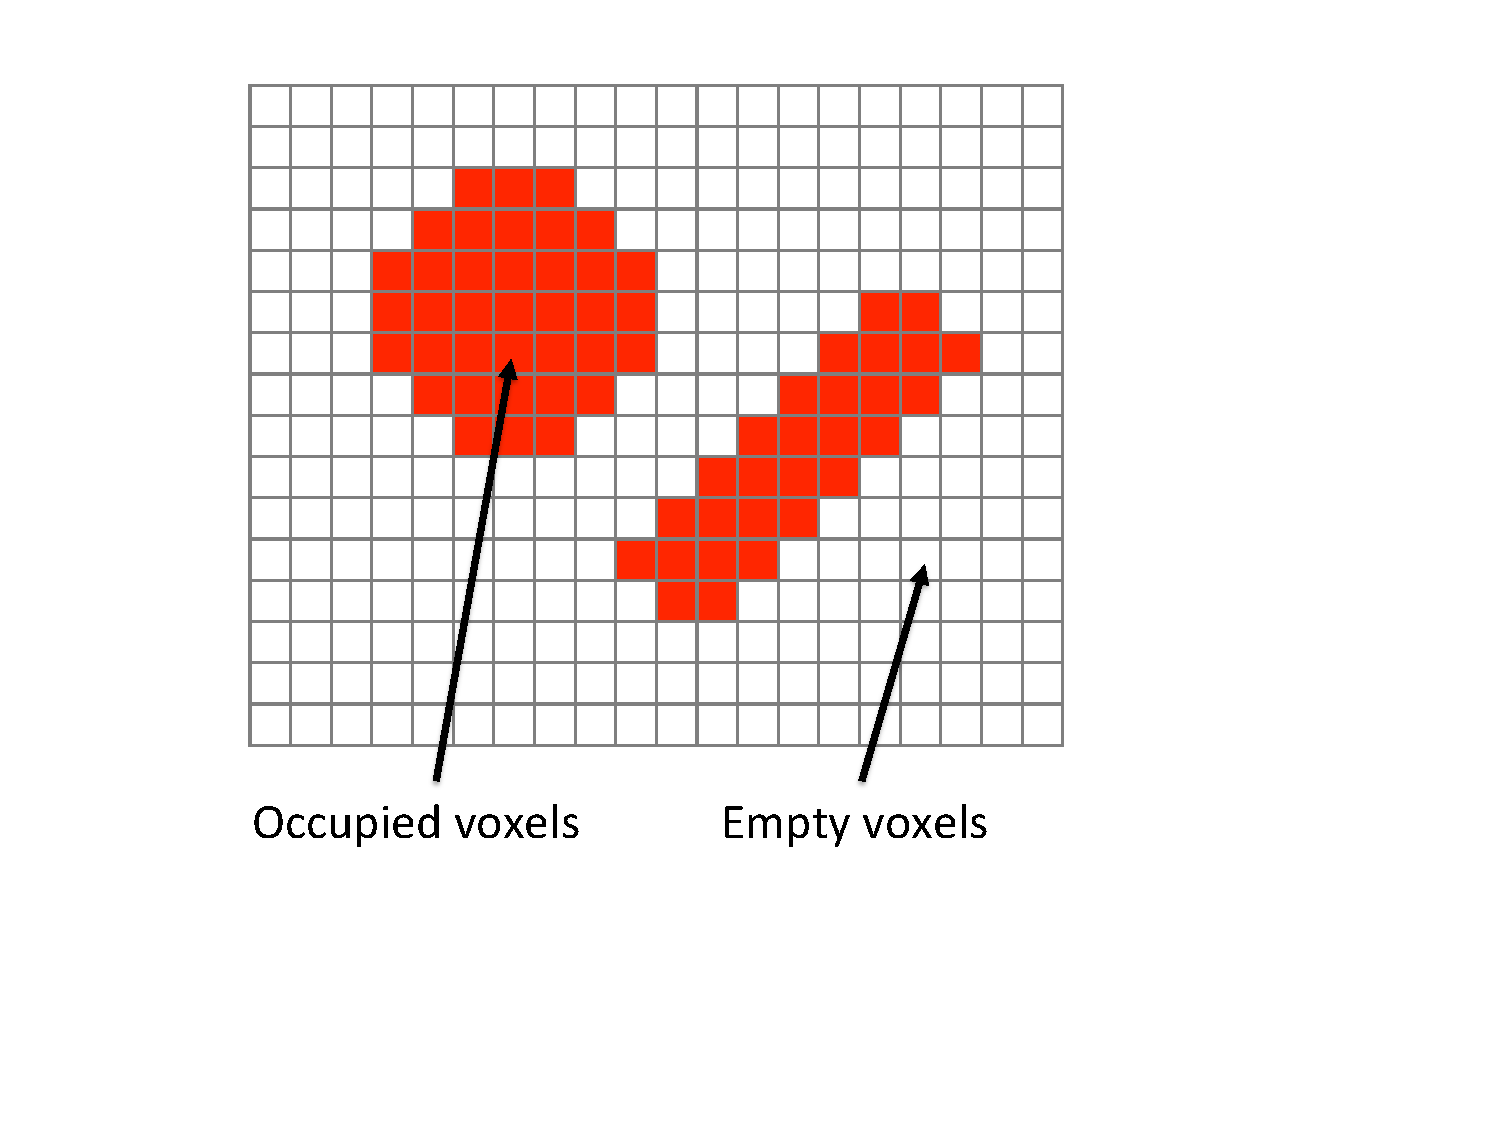
\includegraphics[width=\introsubwidth, clip=true, trim=110 105 205 30]{fig_1}}
        \hfill
    \subfigure[Depth rendering of world]{%
        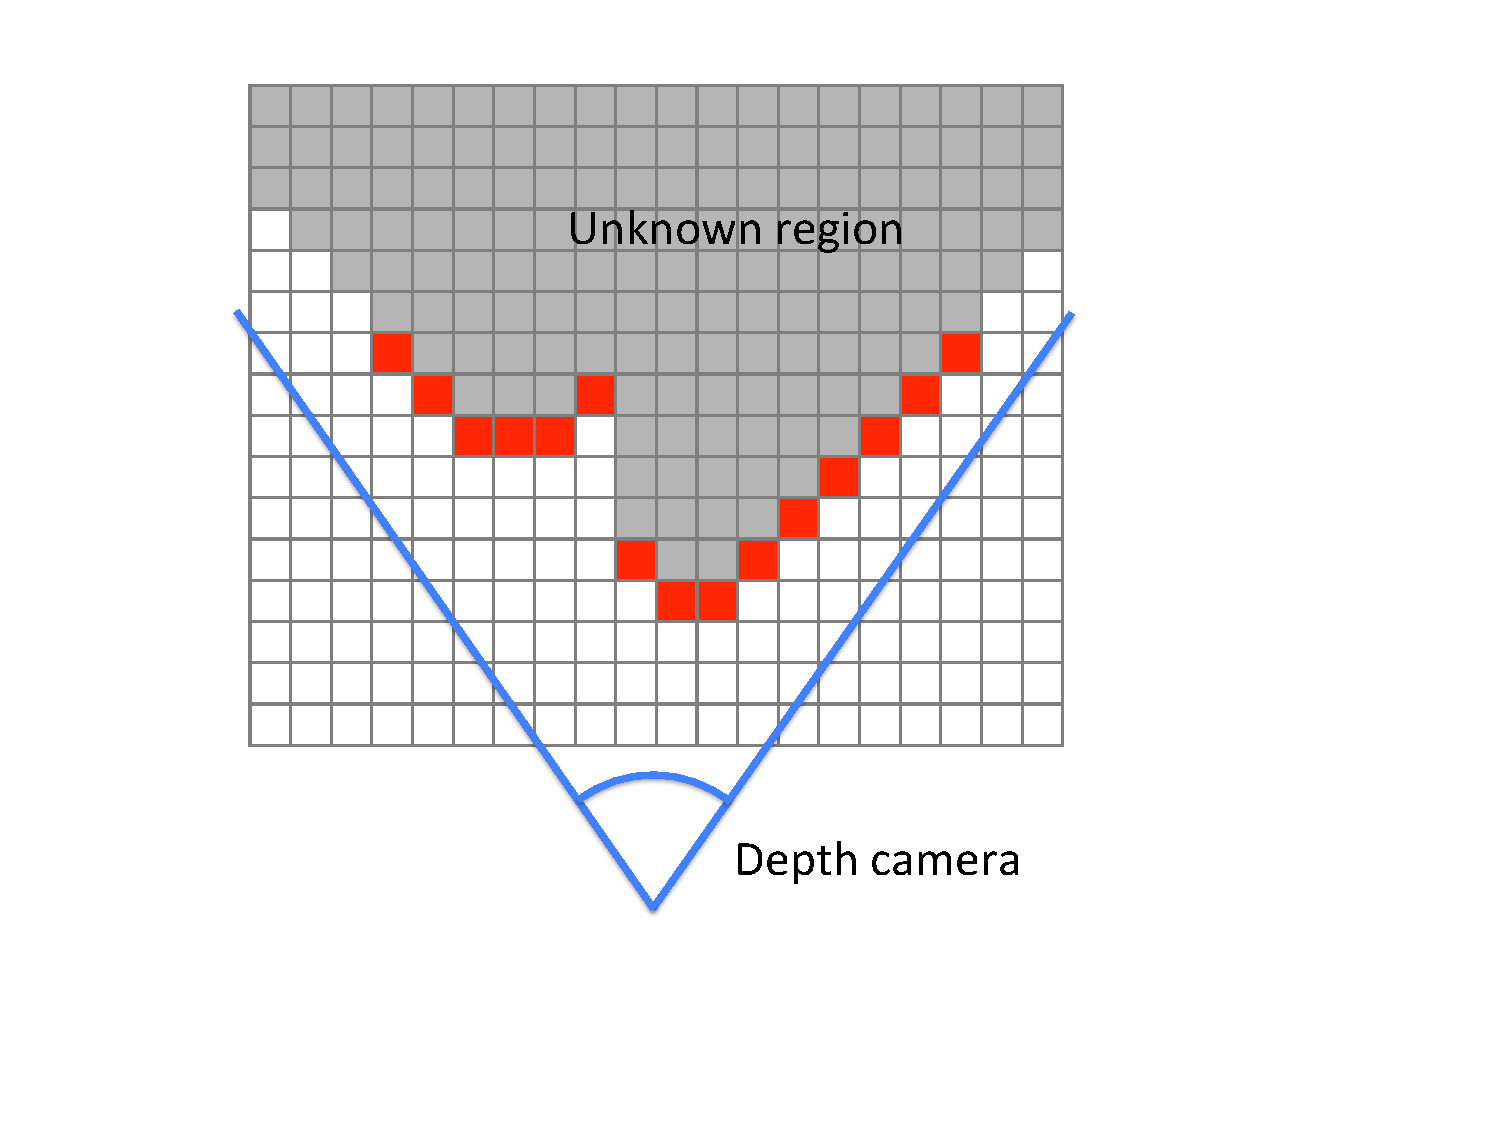
\includegraphics[width=\introsubwidth, clip=true, trim=110 105 205 30]{fig_1b}}
    \caption{
    We assume our world be be made up of voxels, which are either occupied or empty (vacant). 
    A coarse 2D representation of this is shown in (a). 
    When rendered by a depth camera, only the first visible voxel along each ray is rendered.
    This leaves a region of unknown occupancy extending beyond the depth surface (b).
    The aim of our algorithm is to predict the state of the voxels in this unknown region.}%
    \label{fig:intro}
\end{figure}

%%%%%%%%%%%%%%%%%%%%%%%%%%%%%%%%%%%%%%%%%%%%%%%%%%%%%%%%%%%%%%
\subsection{Our approach and contributions}
%%%%%%%%%%%%%%%%%%%%%%%%%%%%%%%%%%%%%%%%%%%%%%%%%%%%%%%%%%%%%%

In this paper we take a data-driven approach to estimating the missing geometry of a scene.
Unlike many papers which tackle this as a mesh completion problem \cite{schnabel-eurographics-2009, ju-cst-2009, silberman-eccv-2014}, we directly tackle the problem by predicting voxel occupancy:
The input to our algorithm is a single depth image, while the output is an estimate of the occupancy of every voxel within the camera frustum.

While some previous work on voxel occupancy prediction incorporates semantics, \eg \cite{kim-iccv-2013, shen-tog-2012, cocias-cgvcv-2013} we are able to predict shape irrespective of recognition of semantic class.
We take inspiration from recent work which has segmented objects from images using silhouettes learned from different object classes \cite{kim-eccv-2012};
their work showed that shape transcends class boundaries, enabling shape predictions to be made regardless of the accuracy of semantic classifiers.
Because we care about shape and voxel occupancy rather than semantic understanding, we are free to use training objects which differ in semantic labelling from the objects being modelled in the scene.
This is key to our approach; we are not reasoning about semantics of objects, but instead about the shape of objects and scenes.

%\paragraph{Aim of the system and overview}
Given a single RGBD image, our system predicts whether each voxel in the scene is occupied by a solid impermeable object, or free and empty. 
In effect, we predict the voxelised occupancy grid of KinectFusion \cite{izadi-uist-2011}, but having been given only a single view of the scene instead of multiple views.

We achieve this by learning a mapping from local and novel semi-regional features to a voxel occupancy in the region of a query point, using a large collection of training objects and scenes.

Our key contributions are:

\begin{itemize}
\item \emph{Voxlets}, a representation of voxel occupancy in the region of a point in a scene. We learn a dictionary of voxlets from training data, and at test time they are able to make structured predictions about occupancy in the region of a query point.
\item We introduce a novel feature representation for a point in a depth image, which captures both local and region-level shape while respecting occlusions.
%\item Use of training data to allow our method to accurately complete detailed shapes.
\end{itemize}


%%%%%%%%%%%%%%%%%%%%%%%%%%%%%%%%%%%%%%%%%%%%%%%%%%%%%%%%%%%%%%
\subsection{Prior work}
%%%%%%%%%%%%%%%%%%%%%%%%%%%%%%%%%%%%%%%%%%%%%%%%%%%%%%%%%%%%%%

Excluding work that makes use of highly specialist hardware, \eg \cite{velten-nature-2012}, most prior work in the area of completing missing data can be categorised according its application domain (\eg meshes \cite{schnabel-eurographics-2009, ju-cst-2009}, 2D images \cite{gupta-cvpr-2011} or depth images \cite{shen-tog-2012}).

\paragraph{Taxonomy of related works}
\note{
Previous works on completion could be categorised according to:
\begin{itemize}
\item their application domain, \ie mesh, 2D photo or voxel. 
\item whether they aim for aesthetic or absolute accuracy.
\item whether they take a data-driven approach or make use of heuristics.
\item if data used for completion come from within the same scene (\eg symmetry), from other scenes (\eg data-driven) or using heuristics.
\end{itemize}
Would be nice to try to make use of these (or other) axes of variation in the writeup, to try to spin some sort of narrative through this section.
}

\paragraph{Semantics}
If prior knowledge is available about the objects present in the scene in the form of 3D models, then an instance-level model can be fitted to the scene giving a good recovery of missing geometry \cite{hinterstoisser-accv-2012, drost-3dimpvt-2012, rusu-iros-2010}.
Many works focus on the problem of where an exact match is not present in the training set.
\cite{shen-tog-2012} complete the missing region of a single object using an assembly of parts from several different models a CAD database, enabling them to model the shape of objects which have not been seen at training time.
In a more general setting, \cite{cocias-cgvcv-2013} enable a class-specific primitive to deform to the shape of an object in a scene, while \cite{prisacariu-iccv-2011} represent the space of shape within a class with a manifold model which can be fitted to the image to infer missing data.
All these methods, however, rely on both the availability of some form of class-level model, and the accuracy of a detector to discover the object in the scene.

\paragraph{Symmetry}
Where we can accurately detect symmetry it is possible to make use of this to complete some types of objects (\eg \cite{law-cviu-2010, thrun-iccv-2005, kroemer-humanoids-2012}). 
Using symmetry for object completion is brittle---an incorrectly guessed symmetrical transform can lead to a catastrophic mis-estimate of geometry---and symmetry is only present in a subset of objects in our world.

\paragraph{Reasoning in 3D}
Fitting bounding boxes is a popular method to explain the arrangement of objects in a scene.
Recent work has successfully incorporated high-level information such as gravity and stability
 \cite{shao-siggraphasia-2014, jia-cvpr-2013}, and made use of training data to accurately detect bounding box locations \cite{hedau-cvpr-2012}.
 Gupta \ea \cite{gupta-cvpr-2011} estimate voxel occupancy from a 2D image, using the clutter detection method of \cite{hedau-iccv-2009}. This occupancy prediction is highly noisy, so is regularised using cuboid `bounding box' hypotheses.
The problem with all these bounding box style methods is that they give very coarse shape information; only a small subset of objects have a nice cuboid shape.


\note{No narrative yet for these:}
\begin{itemize}

\item Kim \ea \cite{kim-iccv-2013} use a CRF model over a voxel representation of a scene to simultaneously predict occupancy, visibility and semantical labelling of voxels from an RGBD image. 
For training, they use manually labelled top-down views of the scene. 
Their prediction of occupancy, however, is really just a Gaussian model. 
Their final labellings found from graph cuts over the CRF. 
They make the observation that the noisy observed values from a Kinect sensor cannot be relied upon and may need cleaning up.

\item Silberman \ea \cite{silberman-eccv-2014} complete meshes from partial Kinect Fusion reconstructions, \eg behind items of furniture.
They use this for augmented realist situations, \eg allowing balls to bounce off floor in unseen areas.
They detect planes in the voxelised representation of the scene, and complete their contours in 2D using a novel CRF method.


\item Fouhey \ea \cite{fouhey-iccv-2013} use the NYU dataset of RGBD images to learn how to predict the normal orientations for each pixel of an input RGB image. 
In our case we are tackling a similar problem at a higher level --- we take RGBD as input, and aim to predict the full geometry of the scene.

\item \cite{guo-iccv-2013} use a single RGBD image to estimate the location and extent of the \emph{support surfaces} (\eg tabletops) in the scene. They do this by processing and analysing the geometry, before finally fitting shapes to the hypothesised support regions. 
\end{itemize}
%\note{They provide boxy user-annotated 3D reconstructions of the full 3D space of the NYU dataset images, which could become useful for our work.}


\paragraph{Image completion and super-resolution}
Image completion works such as \cite{hays-siggraph-2007, criminisi-cvpr-2003}, 
typically use data-driven approaches as it is very difficult to form true generative models over image appearance.
For example, \cite{hays-siggraph-2007} look up possible completion regions in a large database of similar images, while \cite{criminisi-cvpr-2003} in-paint by selecting and combining multiple plausible patches from other regions of the input image.
This differs from our task as image completion typically aims for a visually plausible output irrespective of the accuracy compared to ground truth.
Similar to image \emph{completion} is image \emph{super-resolution}, \eg \cite{macaodha-eccv-2012}. 
This, like our problem, is ill-posed and relies on the repeatability and predictability of the world in order to improve the local geometry of an image.


%%%%%%%%%%%%%%%%%%%%%%%%%%%%%%%%%%%%%%%%
\paragraph{Primitive-based techniques}
There is lots of work on primitive-based techniques to recover the shape and pose of objects; see the related work of \cite{fouhey-iccv-2013} for a good overview.
`Geons' are proposed by \cite{bieberman-rbc-1987} as a set of 3D primitives used for human image understanding. These primitives, such as cylinders and cuboids, must be accurately detected in order to be used in computer vision, and are ultimately a poor representation of the range of shapes present in our world \note{???}.

The typical approach for the use of primitives in vision is to find a mapping from feature space to a label space, where the feature space is a point on an input image and the label space describes a range of world states. 
Feature space is typically limited to an image patch, while the label space may be surface normals \cite{fouhey-iccv-2013}, human poses \cite{bourdev-iccv-2009}, etc.
A question that arises is: How to form the set of primitives?
\cite{bourdev-iccv-2009} do a sort of clustering of their human poses (after aligning in 3D space), while \cite{fouhey-iccv-2013} take perhaps a more principled approach, using a SVM-like formulation to find primitives which are both discriminative in feature space and informative in label space.








%In effect we are hypothesising that any two rays that have a similar appearance from one angle are likely to share similarities in shape in the unobserved regions of the scene.

%In this respect we take inspiration from \cite{kim-eccv-2012}, where silhouettes from training objects are used to segment other objects from different classes.


%Occlusions and occlusion boundaries are a natural result of this projection from world space into image space.
%While often ignored or treated as a `nuicence', recently works have made explicit use of occlusion boundaries \cite{hoiem occlusion boundaires, segmenting simple objects}.

%Going from 2\textonehalf D to a full 3D representation is a challenging problem.
%Typically this has been approached by fusing together images from multiple viewpoints \cite{izadi-uist-2011}.

%Our world is naturally fully three-dimensional: We can think of every point in space as either being `occupied' by impenetrable solid matter, or as being `vacant', \ie transparent.
%A traditional camera image takes this 3D world and projects it onto a 2D plane.
%A great deal of information is lost in the process, as objects are flattened and occlusions prevent points behind those immediately visible to the camera ray from being observed. %, losing a whole dimension in the process.

%In recent years there have been great advances making affordable `3D' sensors available to capture a more complete representation of the world; these cameras, however, are still hampered by occlusions and technically only capture a 2\textonehalf D image.

%In many applications of depth cameras, however, it is not possible to gain a full view of all areas of the scene.


% \begin{quote}
% Voxel occupancy is one approach for reconstructing the 3-dimensional shape of an object from multiple views. In voxel occupancy, the task is to produce a binary labeling of a set of voxels, that determines which voxels are filled and which are empty.
% \cite{snow-cvpr-2000}
% \end{quote}

%%%%%%%%%%%%%%%%%%%%%%%%%%%%%%%%%%%%%%%%%%%%%%%%%%%%%%%%%%%%%%
\subsection{Problem statement}
%%%%%%%%%%%%%%%%%%%%%%%%%%%%%%%%%%%%%%%%%%%%%%%%%%%%%%%%%%%%%%

We assume the 3D geometry of a scene to be made up of a dense set of voxels $\voxelgrid = \{\voxel_\voxidx\}$, where each $\voxel_\voxidx \in [0, 1]$ is a binary variable which takes the value $0$ if the voxel is vacant, and $1$ if it is occupied, and $\voxidx = (\voxelidxs)$  denotes the index coordinates of voxel $\voxidx$ in the grid.
An index location $\voxidx$ can be mapped to 3D world space under the affine transformation $\voxelgridtoworld$.

We treat a voxel as occupied if you cannot view its state from a camera moving around the scene from its start position.
So a voxel inside a closed cardboard box, while void of solid object, would be considered occupied.
On the other hand, a voxel on the inside of a cardboard box open at the top would be considered unoccupied.

Our scene geometry $\voxelgrid$ is then captured in a single static depth image $\rgbdimage$ by a camera with extrinsics $\extrinsics$ and intrinsics $\intrinsics$. 
Assuming perspective projection, the center location of each voxel projects into the camera to a position of:
\begin{equation}
[u, v, d]^T = \intrinsics \extrinsics \voxelgridtoworld [\voxelidxs]^T,
\end{equation}
where $(u,v)$ the position of the voxel in image coordinates and $d$ is the  perpendicular distance from the camera centre to the voxel.
Finally, the value of each pixel $(u^*, v^*)$ in the depth image $\rgbdimage$ is given by the depth to the first occupied voxel along the camera ray:
\begin{equation}
\rgbdimage(u^*,v^*) = \min_\voxidx \left\{ d_{\voxidx} : v_{\voxidx} = 1, \lfloor u_{\voxidx} \rfloor = u^*, \lfloor v_{\voxidx} \rfloor = v^* \right\}.
\label{eqn:minimisation}
\end{equation}
%_{world \rightarrow camera} H_{grid \rightarrow world}

The $\min_\voxidx$ in (\ref{eqn:minimisation}) is the manifestation of occlusion: Each ray from the camera stops at the first occupied voxel it reaches.
The aim of our algorithm is to recover $\voxelgrid$ given $\rgbdimage$.


%http://scholar.google.co.uk/scholar?safe=off&espv=2&bav=on.2,or.r_cp.r_qf.&bvm=bv.75775273,d.ZWU,pv.xjs.s.en.CtdJ7drbKko.O&ion=1&biw=1164&bih=816&um=1&ie=UTF-8&lr=&cites=16286130882256685425


\begin{figure}
  \centering 
  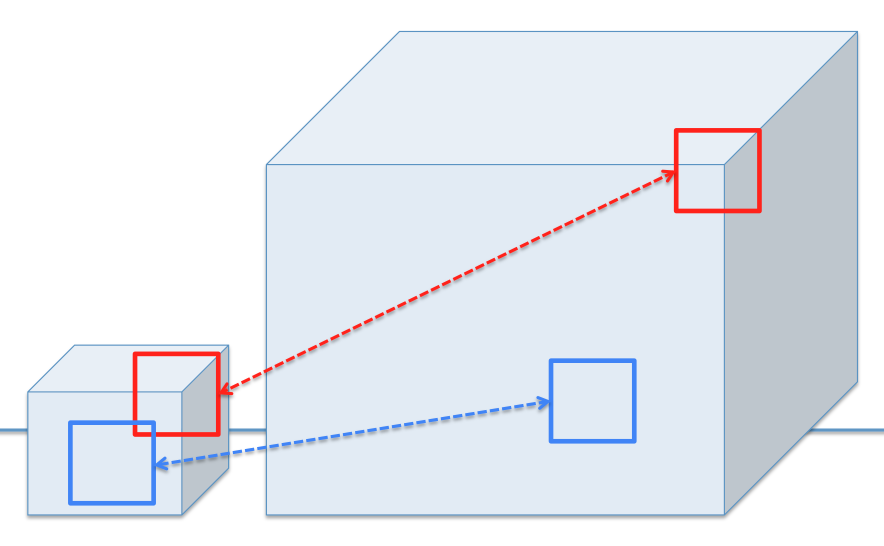
\includegraphics[width=0.9\columnwidth]{patch_sizes.png}
      
  \caption{Local, patch-type features do not give enough information to accurately predict depth. Here, two pairs of patches are marked. Each item in these pairs have identical local appearance. However, the thickness of the object at each patch location is very different. We use this to motivate the spider feature.}
\end{figure}


% %%%%%%%%%%%%%%%%%%%%%%%%%%%%%%%%%%%%%%%%%%%%%%%%%%%%%%%%%%%%%%%%%%%%%%%%%%%%%%%%
\section{Notes}
% %%%%%%%%%%%%%%%%%%%%%%%%%%%%%%%%%%%%%%%%%%%%%%%%%%%%%%%%%%%%%%%%%%%%%%%%%%%%%%%%
Just some notes of things to also include:

\begin{itemize}
\item Literature on surface descriptions (normal estimation? depth/sliding window?)
\item Combine all the motivational images for the spider feature into one...
\begin{itemize}
\item Patch based motivation
\item Occlusion based motivation
\end{itemize}
\item Combine all the describing images for the spider feature into one...
\begin{itemize}
\item View of 3D scene with p, e etc
\item Slice through (fig 5 currently I think)
\item Cobweb feature...
\end{itemize}
\end{itemize}


% %%%%%%%%%%%%%%%%%%%%%%%%%%%%%%%%%%%%%%%%%%%%%%%%%%%%%%%%%%%%%%%%%%%%%%%%%%%%%%%%
\section{Approach overview}
% %%%%%%%%%%%%%%%%%%%%%%%%%%%%%%%%%%%%%%%%%%%%%%%%%%%%%%%%%%%%%%%%%%%%%%%%%%%%%%%%

Our approach is somewhat inspired by patch-based methods used for superresolution or similar of depth images. 
However, as we are predicting in 3D space we introduce \emph{voxlets}.

% Overview of the method --- Figure \ref{fig:pipeline}.
% General motivation for method. Do not want to rely on having exact matches in training set. 
% Instead, want to find a collection of good matches in the training set which, when combined, will give a sensible prediction of the voxel occupancy.
% We take a RANSAC-style approach to finding basis shapes: first we \emph{propose} a set of candidate shapes which roughly match the scene, before we next \emph{re-weight} these candidates according to how well they match the scene geometry. 

\remove{The aim of our thickness prediction function is to map a point $\point$ in the image to a scalar thickness $t$.}


%%%%%%%%%%%%%%%%%%%%%%%%%%%%%%%%%%%%%%%%%%%%%%%%%%%%%%%%%%%%%%%%%%%%%%%%%%%%%%%%%
\section{Discontinuity discovery}
%%%%%%%%%%%%%%%%%%%%%%%%%%%%%%%%%%%%%%%%%%%%%%%%%%%%%%%%%%%%%%%%%%%%%%%%%%%%%%%%%

Describe here:
\begin{itemize}
\item Reprojecting the depth image into the colour camera
\item Smoothing - both citations
\item Types of edges (depth, colour, occluding etc)
\item Our method for depth edges
\item motivation - why do we care about occlusions?
\end{itemize}

We reason that discontinuities in depth images can be assigned a direction: one side of each edge is the occluder, the other is the occludee. 
We can compute the gradient of the depth edges using PCA on the edge pixels in image space.
We ensure that the final gradient at each edge pixel points in the direction of the occluded side.

We can then use the occlusion information in our feature computations---see for example figure \ref{fig:occluded_region}.

\begin{figure}
    \centering 
    \subfigure[]{%
        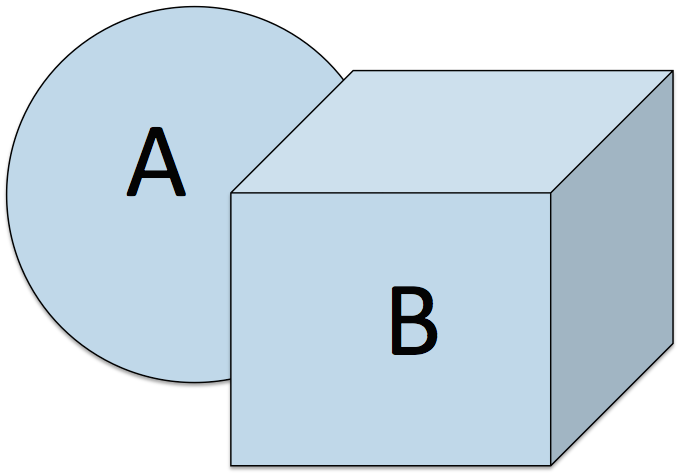
\includegraphics[width=0.45\columnwidth]{occlusion_a}}
        \hfill
    \subfigure[]{%
        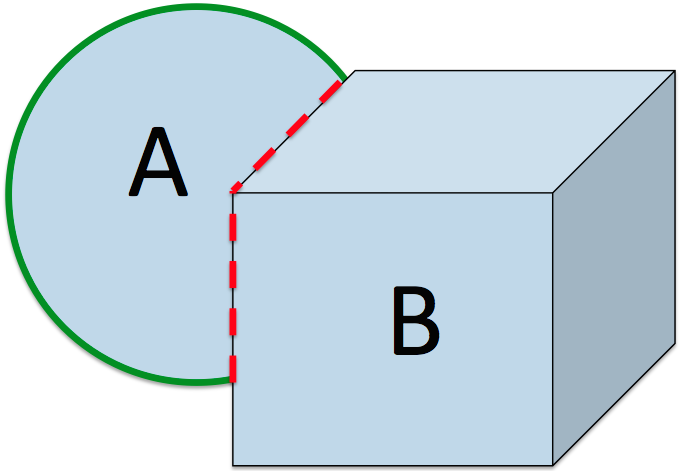
\includegraphics[width=0.45\columnwidth]{occlusion_b}} \\
    \caption{Where edges occur as a result of occlusion boundaries, the direction of the edge is important. The edge bounding region A can be divided into an \emph{occluding} portion (solid green) and an \emph{occluded} portion (dashed red).
    We can make a reasonable assumption that region A may extend behind object B past the occluded edge---however, region A cannot continue sideways beyond its occluding edge.}
    \label{fig:occluded_region}
\end{figure}



%%%%%%%%%%%%%%%%%%%%%%%%%%%%%%%%%%%%%%%%%%%%%%%%%%%%%%%%%%%%%%%%%%%%%%%%%%%%%%%%%
\section{Voxlets}
%%%%%%%%%%%%%%%%%%%%%%%%%%%%%%%%%%%%%%%%%%%%%%%%%%%%%%%%%%%%%%%%%%%%%%%%%%%%%%%%%


%%%%%%%%%%%%%%%%%%%%%%%%%%%%%%%%%%%%%%%%%%%%%%%%%%%%%%%%%%%%%%%%%%%%%%%%%%%%%%%%%
\section{Feature representation}
%%%%%%%%%%%%%%%%%%%%%%%%%%%%%%%%%%%%%%%%%%%%%%%%%%%%%%%%%%%%%%%%%%%%%%%%%%%%%%%%%

%\section{Predicting thickness}

Our method is to use local and regional features extracted from the image around $\point$ to predict the thickness of the object at that point.
We use two novel features, which we describe in detail here. See also figure \ref{fig:features}.

\newcommand{\subwidth}{0.32\columnwidth}
\begin{figure*}
    \centering 
    \subfigure[Spider feature]{%
        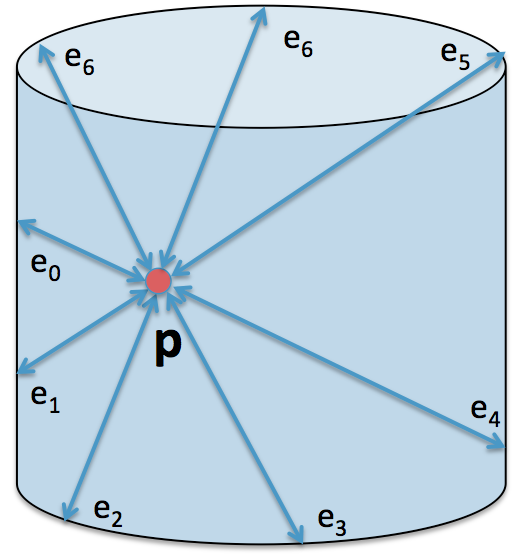
\includegraphics[width=\subwidth]{02_spider}}
        \hfill
    \subfigure[Occluded spider]{%
        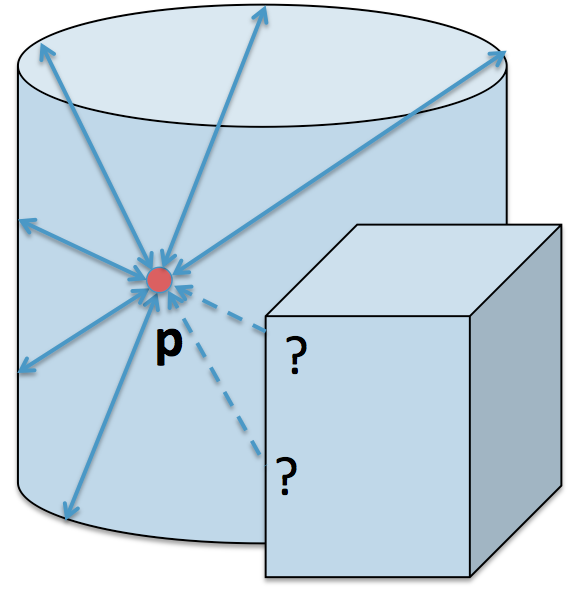
\includegraphics[width=\subwidth]{04_spider_occ}
        \label{fig:features:occluded_spider}}
        \hfill
    \subfigure[Cobweb feature]{%
        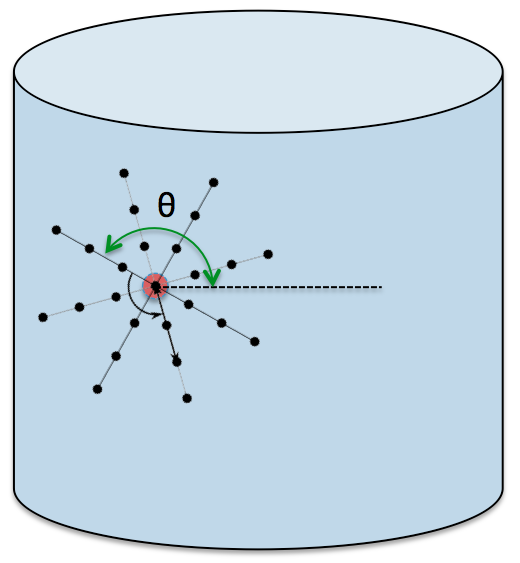
\includegraphics[width=\subwidth]{05_cobweb}}
        \hfill
    \caption{
    %(a) Each point on a depth image has an angle $\theta$ associated, which represents the direction of gradient of the depth. 
    (b) The spider features measure the distance between $\point$ and the edge points $e_{1, \cdots, 7}$.
    %(c) Because the spider features are computed relative to $\theta$, the resultant feature vector is invariant to object rotations in the camera plane.
    (d) Where the spider line emitted from $\point$ first hits an occluded edge, only a \textit{minimum} extent is known---this case is denoted as \texttt{?} in this figure.
    (e) The cobweb feature measures the difference in depth between $\point$ and a set of points in the near vicinity of $\point$, arranged in a cobweb shape.}%
    \label{fig:features}
\end{figure*}


\begin{figure}
    \centering 
    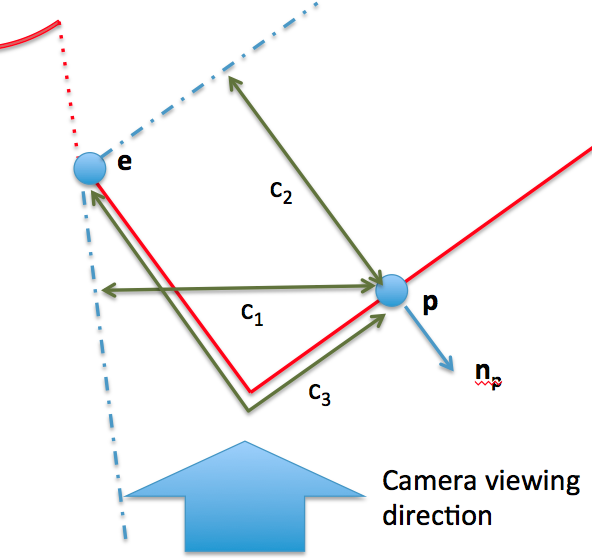
\includegraphics[width=1.0\columnwidth]{compass_features}
    \caption{We compute three flavours of compass features, which measure the distance between $\mathbb{p}$ and the edge point $\mathbb{e}$ in different ways. $c_1$ is the distance perpendicular to the camera direction; $c_2$ measures the depth of the object perpendicular to the normal at $\mathbb{p}$; while $c_3$ is the geodesic distance between $\mathbb{p}$ and $\mathbb{e}$.}
    \label{fig:compass_features}
\end{figure}


%%%%%%%%%%%%%%%%%%%%%%%%%%%%%%%%%%%%%%%%%%
\subsubsection{Cobweb feature }
\note{Name up for debate!}
The cobweb feature is a simple pairwise feature, inspired by recent work such as \cite{shotton-cvpr-2011}, capturing the surface shape in the immediate vicinity of $\point$.
\begin{align}
f(u, v, \psi, t) &= \rgbdimage(u, v) - \rgbdimage(a, b) \\
a &= \left\lfloor u + M(t)  \sin(\psi) \right\rceil \\
b &= \left\lfloor v + M(t)  \cos(\psi) \right\rceil
\end{align}
where $M(x) = fx / \rgbdimage(u, v)$ uses the focal length $f$ to map a distance in world space to a pixel offset. For our experiments we compute the cobweb feature for all combinations of $\psi = [0\degree, 45\degree, \ldots, 315\degree]$ and $t = [0.02m, 0.04m, 0.06m]$.
The final cobweb feature is therefore 24-dimensional.
%Note also: ``If an offset pixel lies on the background or outside the bounds of the image, the depth probe dI (x0) is given a large positive constant value''.

%%%%%%%%%%%%%%%%%%%%%%%%%%%%%%%%%%%%%%%%%%
\subsubsection{Spider features }
\note{Name up for debate!}

\note{Lots of papers \eg microsoft use local features in region of point. For thickness this doesn't cut the mustard, so we augment with region features. However, most region features ignore occlusions. We don't.}

The cobweb feature is 

The spider feature captures the size and shape of the region in which $\point$ resides. 
Rather than explicitly computing region-level features, however, which may suffer from poor segmentations (and the problem with occlusion), we compute these features capturing the region's shape at the point level. 
We first compute an edge map for the image.
We again consider the set of angles $\phi$. Starting from $\point$, we cast a Bresenham line along the depth image until it hits an edge. 
We denote the point at which the edge was hit as $\point_{e}$.

For each line cast, we store
a) the geodesic distance between $\point$ and $\point_{e}$ along the depth surface, and 
b) the 3D distance between $\point$ and $\point_{e}$ along the direction of the normal at $\point$. (In practice, we take the point 95\% of the way between $\point$ and $\point_{e}$ in image space, as this helps to prevent problems with poor quality edge data).

The spider feature is therefore 16-dimensional.

While it captures a wide range of information about the region within which a point resides, the spider feature is extremely efficient to compute.
This is mainly due to the additive nature of the feature: The spider feature in direction $0\degree$ at $(i, j)$ can be computed from summing a small fraction 
We can compute the 16D spider feature for every point in a $640\times480$ image in less than 0.01s using unoptomised C++ code; we would expect a significant speedup were this to be implemented on a GPU.

\subsubsection{Occluded spider features}

We explicitly handle occlusion in the spider features. Where the spider feature first hits an occluded edge rather than an occluding edge, the true size of the object in that dimension is unknown (see figure \ref{fig:features:occluded_spider}).
However, we do have a \textit{minimum} size in that direction.
%We explicitly encode this unknown value --- in practice with \texttt{NaN} --- and the Random Forest can then make a sensible decision about what to do with it.

% \begin{figure}
%     \centering% 
%     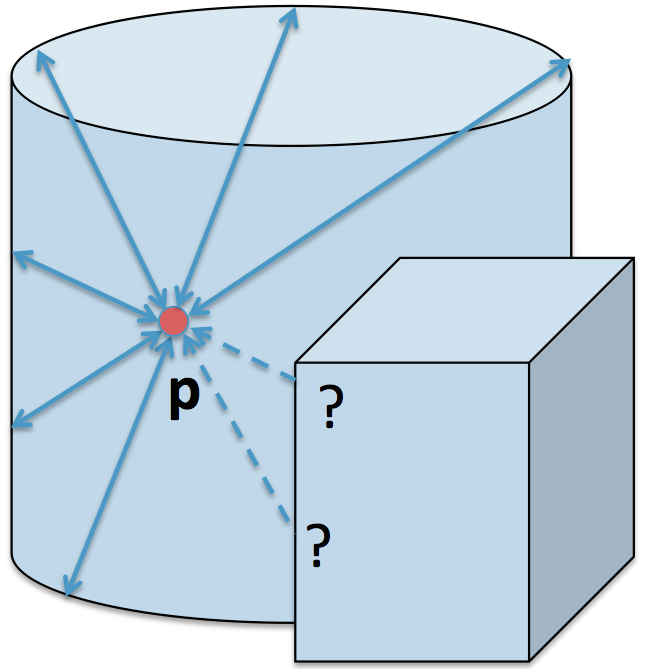
\includegraphics[width=0.7\columnwidth]{occlusion_spider.png}% 
%     \figcaption{The spider feature extends lines from $\point$ to the first occluding edge found along the path. Internal edges (e.g. those found in RGB space) are ignored. Where the line first hits an occluded edge, the true extent is unknown --- this case is denoted as \texttt{?} in this figure.}% 
%     \label{fig:occluded_spider}% 
% \end{figure}



%We train a Random Forest using a total of 1,000,000 training examples extracted from 1,600 CAD models, each rendered from 42 different angles.

%\begin{figure}
%    \centering% 
%    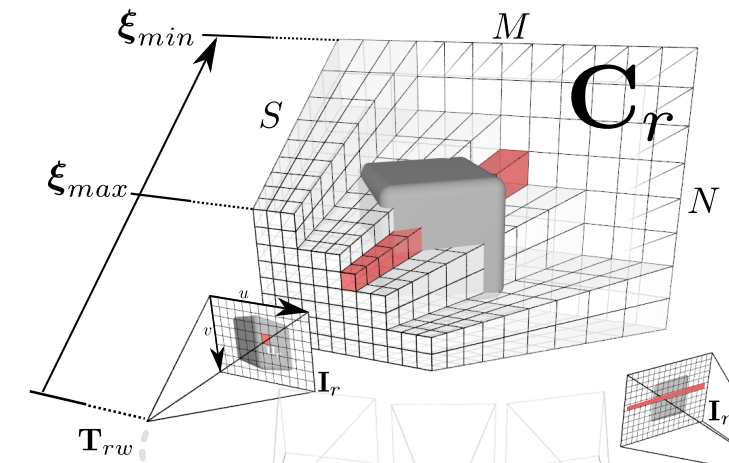
\includegraphics[width=1.0\columnwidth]{dtam_voxels.png}% 
%    \figcaption{The warped voxelisation we make of our scene.
%    The voxel space is a frustum grid, and each voxel is therefore a prismoidal hexahedron.
%    Image from \cite{newcombe-iccv-2011}---I should probably make a similar one.}% 
%    \label{fig:dtam_voxels}% 
%\end{figure}



%%%%%%%%%%%%%%%%%%%%%%%%%%%%%%%%%%%%%%%%%%%%%%%%%%%%%%%%%%%%%%%%%%%%%%%%%%%%%%%%
\section{Regularisation}
%%%%%%%%%%%%%%%%%%%%%%%%%%%%%%%%%%%%%%%%%%%%%%%%%%%%%%%%%%%%%%%%%%%%%%%%%%%%%%%%



%%%%%%%%%%%%%%%%%%%%%%%%%%%%%%%%%%%%%%%%%%%%%%%%%%%%%%%%%%%%%%%%%%%%%%%%%%%%%%%%
\section{Experiments}
%%%%%%%%%%%%%%%%%%%%%%%%%%%%%%%%%%%%%%%%%%%%%%%%%%%%%%%%%%%%%%%%%%%%%%%%%%%%%%%%

\paragraph{Evaluation criteria}
The aim of our algorithm is to accurately classify free space in a scene; therefore, we report the per-voxel ROC curve for the scene, comparing the prediction $\Pr(o)$ with the ground truth occupancy as provided by KinFu.

The shape of the ROC curve is strongly affected by the region over which the evaluation is performed.
If all the voxels between the camera and the depth image are included in the evaluation, the false positive rate becomes very low, as the voxels in the free space between the camera and scene are `easy wins' for the algorithm. We therefore evaluate over all the voxels 


\begin{figure}
    \centering% 
    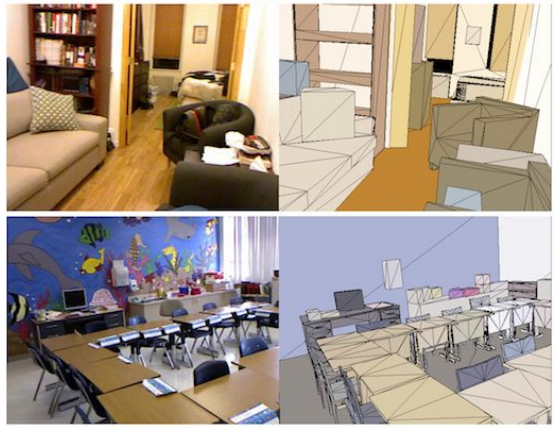
\includegraphics[width=1.0\columnwidth]{guo.png}% 
    \figcaption{Representation of objects in the NYU dataset, provided from \cite{guo-iccv-2013}.
    Not a perfect representation but perhaps reasonable to some extents.}% 
    \label{fig:guo_labels}% 
\end{figure}


\subsection{Database of CAD models}
Use the database from Fisher \ea \cite{fisher-siggraphasia-2012}.
1600 CAD models, each depth-rendered from 42 viewing angles using OpenGL.

\subsubsection{Potential test datasets}
\begin{itemize}
\item Create our own KinFu dataset
\item Kaparthy \ea --- would probably have to re-render their meshes.
Also don't have the TSDF etc. Lots of problems
\item NYU dataset --- classic dataset. Potential ground truth labels from \cite{guo-iccv-2013} (figure \ref{fig:guo_labels}) or \cite{kim-iccv-2013}.
\item \cite{fisher-siggraphasia-2012}, use their synthetic scenes (great for a first pass!)
\end{itemize}

\begin{figure}
    \centering% 
    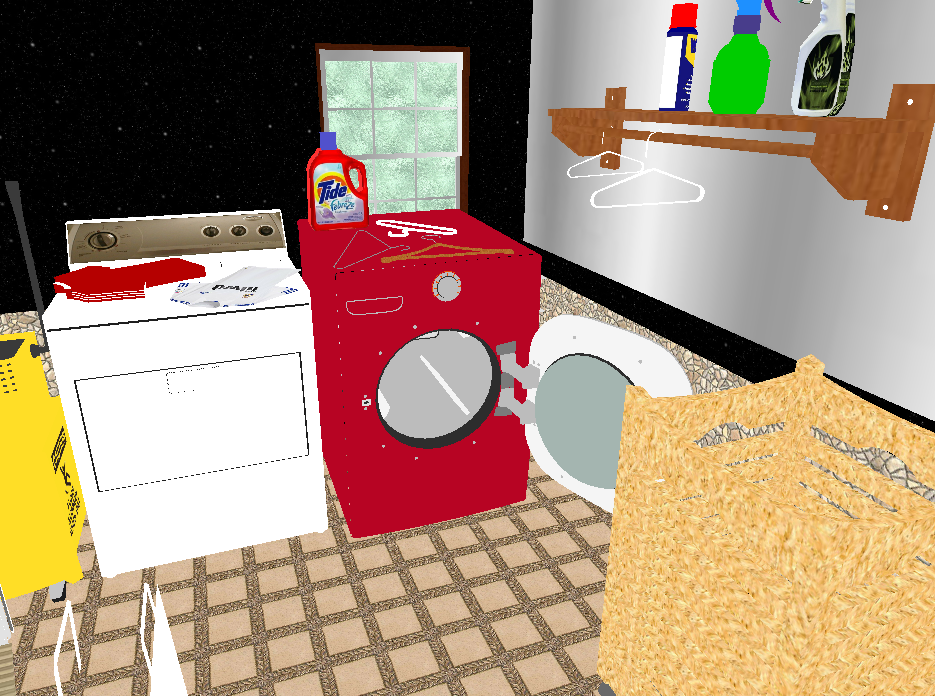
\includegraphics[width=1.0\columnwidth]{synth_scene.png}% 
    \figcaption{One of the user-created synthetic scenes from \cite{fisher-siggraphasia-2012}.}% 
    \label{fig:fisher_scene}% 
\end{figure}

% \section{Acknowledgements}
% Peter Gehler
% Malcolm
% Neill
% Prism group
% Tom
% Peter
% 

{\small
\bibliographystyle{ieee}
\bibliography{bibtex/strings.bib,bibtex/main.bib,bibtex/crossrefs.bib}
}

%\printbibliography


\end{document}